\section{勾配法と誤差逆伝播法}
\textbf{\index{ごさぎゃくでんぱほう(back-propagation)@誤差逆伝播法(back-propagation)}}
\subsection{ニューラルネットワークモデル}
この節では入力層,隠れ層,出力層からなる3層ニューラルネットワークを実装する.
\lstinputlisting[language=julia]{./text/solve-credit-assignment-problem/backpropagation/001.jl}
\lstinputlisting[language=julia]{./text/solve-credit-assignment-problem/backpropagation/002.jl}
mutable struct \jl{NN}を用意し,\textbf{\index{おもみのしょきか(weight initialization)@重みの初期化(weight initialization)}} を行う同名の関数\jl{NN}を用意する.重みの初期化の手法は複数ある(Glorot & Bengio, 2010)が,ここでは重みを$w$として,$w \sim U\left(-1/\sqrt{n}, 1/\sqrt{n}\right)$とする.ただし,$n$は入力ユニット数である.
\subsubsection{Optimizerの作成}
abstract typeとして\jl{Optimizer}タイプを作成する.
\lstinputlisting[language=julia]{./text/solve-credit-assignment-problem/backpropagation/005.jl}
\textbf{\index{かくりつてきこうばいこうかほう(stochastic gradient descent; SGD)@確率的勾配降下法(stochastic gradient descent; SGD)}} を実装する.
\lstinputlisting[language=julia]{./text/solve-credit-assignment-problem/backpropagation/007.jl}
次に\textbf{\index{Adam}} ([Kingma & Ba, 2014](https://arxiv.org/abs/1412.6980)) を実装する.
\lstinputlisting[language=julia]{./text/solve-credit-assignment-problem/backpropagation/009.jl}
\subsubsection{順伝播・逆伝播の実装}
活性化関数を用意する.今回はsigmoid関数のみ使用する.
\lstinputlisting[language=julia]{./text/solve-credit-assignment-problem/backpropagation/011.jl}
$f(\cdot)$を活性化関数とする.順伝播(feedforward propagation)は以下のようになる.


\begin{align}
\text{入力層 : }&\mathbf{z}^{(0)}=\mathbf{x}\\
\text{隠れ層 : }&\mathbf{z}^{(\ell)}=f\left(\mathbf{a}^{(\ell)}\right)\\
&\mathbf{a}^{(\ell+1)}=W^{(\ell+1)}\mathbf{z}^{(\ell)}+\mathbf{b}^{(\ell+1)}\\
\text{出力層 : }&\hat{\mathbf{y}}=\mathbf{z}^{(L)}
\end{align}


逆伝播(backward propagation)


\begin{align}
\text{目的関数 : }&\mathcal{L}=\frac{1}{2}\left\|\hat{\mathbf{y}}-\mathbf{y}\right\|^{2}\\
\text{最急降下法 : }&\Delta W^{(\ell)}=-\eta \frac{\partial \mathcal{L}}{\partial W^{(\ell)}}\\
&\Delta \mathbf{b}^{(\ell)}=-\eta \frac{\partial \mathcal{L}}{\partial \mathbf{b}^{(\ell)}}\\
\text{誤差逆伝播法 : }&\frac{\partial \mathcal{L}}{\partial \hat{\mathbf{y}}}=\frac{\partial \mathcal{L}}{\partial \mathbf{z}^{(L)}}=\hat{\mathbf{y}}-\mathbf{y}\\
&\delta^{(L)}=\frac{\partial \mathcal{L}}{\partial \mathbf{z}^{(L)}} \frac{\partial \mathbf{z}^{(L)}}{\partial \mathbf{a}^{(L)}}=\left(\hat{\mathbf{y}}-\mathbf{y}\right) \odot f^{\prime}\left(\mathbf{a}^{(L)}\right)\\
&\mathbf{\delta}^{(\ell)}=\frac{\partial \mathcal{L}}{\partial \mathbf{z}^{(\ell)}} \frac{\partial \mathbf{z}^{(\ell)}}{\partial \mathbf{a}^{(\ell)}}=\left(W^{(\ell+1)}\right)^\top \delta^{(\ell+1)} \odot f^{\prime}\left(\mathbf{a}^{(\ell)}\right)\\
&\frac{\partial \mathcal{L}}{\partial W^{(\ell)}}=\frac{\partial \mathcal{L}}{\partial \mathbf{z}^{(\ell)}} \frac{\partial \mathbf{z}^{(\ell)}}{\partial \mathbf{a}^{(\ell)}} \frac{\partial \mathbf{a}^{(\ell)}}{\partial W^{(\ell)}}=\delta^{(\ell)}\left(\mathbf{z}^{(\ell-1)}\right)^\top\\
&\frac{\partial \mathcal{L}}{\partial \mathbf{b}^{(\ell)}}=\frac{\partial \mathcal{L}}{\partial \mathbf{z}^{(\ell)}} \frac{\partial \mathbf{z}^{(\ell)}}{\partial \mathbf{a}^{(\ell)}} \frac{\partial \mathbf{a}^{(\ell)}}{\partial \mathbf{b}^{(\ell)}}=\delta^{(\ell)}
\end{align}


バッチ処理を考慮すると,行列を乗ずる順番が変わる.
\lstinputlisting[language=julia]{./text/solve-credit-assignment-problem/backpropagation/013.jl}

\frac{d}{dx} \text{Sigmoid}(x) = \text{Sigmoid}(x) \cdot \left(1 - \text{Sigmoid}(x)\right)

であることに注意.
\subsection{MNIST}
\subsection{Zipser-Andersenモデル}
Zipser-Andersenモデル \cite{Zipser1988-nc} は頭頂葉の7a野のモデルであり,網膜座標系における物体の位置と眼球位置を入力として,頭部中心座標(head centered coordinate)に変換する.隠れ層はPPC(Posterior parietal cortex)の細胞のモデルになっている.
\subsubsection{データセットの生成}
物体位置の表現にはGaussian形式とmonotonic形式があるが,簡単のために,Gaussian形式を用いる.なお,monotonic形式については末尾の補足を参照してほしい.
\lstinputlisting[language=julia]{./text/solve-credit-assignment-problem/backpropagation/017.jl}
入力は64(網膜座標系での位置)+2(眼球位置信号)=66とする.眼球位置信号は原著ではmonotonic形式による32(=8ユニット×2(x, y方向)×2 (傾き正負))ユニットで構成されるが,簡単のために眼球位置信号も$x, y$の2次元とする.視覚刺激は-40度から40度までの範囲であり,10度で離散化する.よって,網膜座標系での位置は$8\times 8$の行列で表現される.位置は2次元のGaussianで表現する.ただし,1/e幅 (ピークから1/eに減弱する幅) は15度である.$1/e$の代わりに$1/2$とすれば半値全幅(FWHM)となる.スポットサイズを$w$,Gaussianを$G(x)$とすると.$G(x+w/2)=G/e$より,$\sigma=\frac{\sqrt{2}w}{4}$と求まる.
\lstinputlisting[language=julia]{./text/solve-credit-assignment-problem/backpropagation/019.jl}
\lstinputlisting[language=julia]{./text/solve-credit-assignment-problem/backpropagation/020.jl}
モデルの定義を行う.
\lstinputlisting[language=julia]{./text/solve-credit-assignment-problem/backpropagation/022.jl}
学習を行う.
\lstinputlisting[language=julia]{./text/solve-credit-assignment-problem/backpropagation/024.jl}
損失の変化を描画する.
\lstinputlisting[language=julia]{./text/solve-credit-assignment-problem/backpropagation/026.jl}
\begin{figure}[ht]
	\centering
	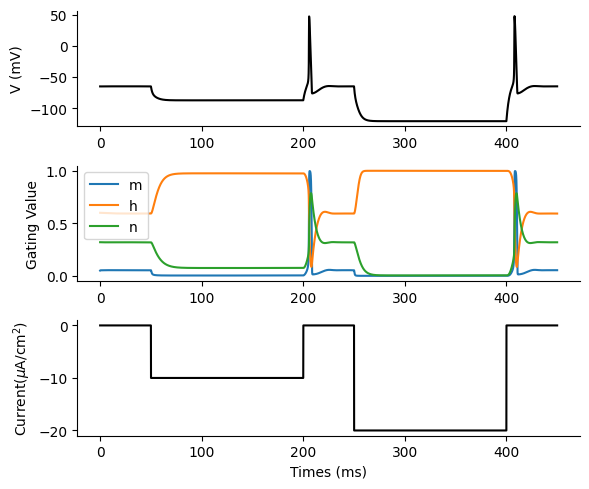
\includegraphics[scale=0.8, max width=\linewidth]{./fig/neuron-model/hodgkin-huxley/cell026.png}
	\caption{cell026.png}
	\label{cell026.png}
\end{figure}
テストデータを用いて,出力を確認する.
\lstinputlisting[language=julia]{./text/solve-credit-assignment-problem/backpropagation/028.jl}
\begin{figure}[ht]
	\centering
	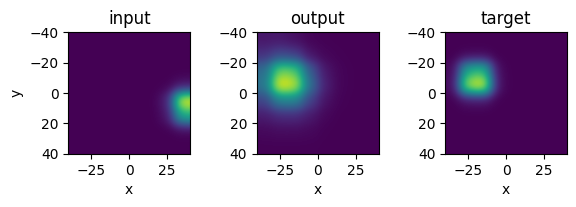
\includegraphics[scale=0.8, max width=\linewidth]{./fig/solve-credit-assignment-problem/backpropagation/cell028.png}
	\caption{cell028.png}
	\label{cell028.png}
\end{figure}
重み\jl{W1}におけるゲインフィールドの描画を行う.
\lstinputlisting[language=julia]{./text/solve-credit-assignment-problem/backpropagation/030.jl}
\begin{figure}[ht]
	\centering
	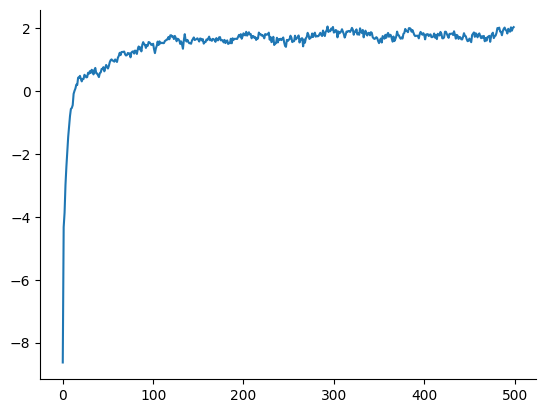
\includegraphics[scale=0.8, max width=\linewidth]{./fig/bayesian-brain/mcmc/cell030.png}
	\caption{cell030.png}
	\label{cell030.png}
\end{figure}
\subsection{補足:Monotonic formatによる位置のエンコーディング}
monotonic形式を入力の眼球位置と出力の頭部中心座標で用いるという仮定には,視覚刺激を中心窩で捉えた際,得られる眼球位置信号を頭部中心座標での位置の教師信号として使用できるという利点がある.([Andersen & Mountcastle, J. Neurosci. 1983](https://pubmed.ncbi.nlm.nih.gov/6827308/))では Parietal visual neurons (PVNs)の活動を調べ,傾き正あるいは負.0度をピークとして減少あるいは上昇の4種類あることを示した.前者は一次関数 (とReLU関数) で記述可能である.
\lstinputlisting[language=julia]{./text/solve-credit-assignment-problem/backpropagation/032.jl}
\begin{figure}[ht]
	\centering
	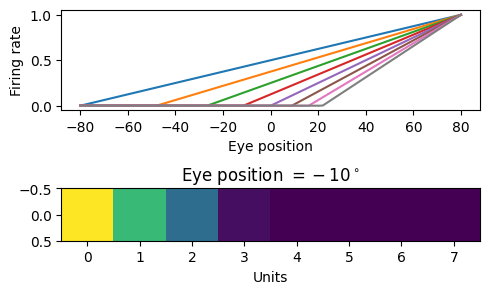
\includegraphics[scale=0.8, max width=\linewidth]{./fig/solve-credit-assignment-problem/backpropagation/cell032.png}
	\caption{cell032.png}
	\label{cell032.png}
\end{figure}
